\section{Auswertung}
\label{sec:Auswertung}

Die Graphen werden sowohl mit Matplotlib \cite{matplotlib} als auch NumPy \cite{numpy} erstellt. Die Fehlerrechnung wird mithilfe von Uncertainties \cite{uncertainties} durchgeführt.\\
In Tabelle \ref{tab:V} sind die Volumina der Bauteile eingetragen und bei welcher Messung diese Verwendet werden. TL bezieht sich auf die Leckratenmessung der Turbopumpe, TE auf die Evakuierungskurve der Turbopumpe, DL auf die Leckratenmessung der Drehschieberpumpe und DE auf die Evakuierungskurve der Drehschieberpumpe. Die Zahl in Klammern hinter diesen Bezeichnungen gibt eine mögliche häufigere Verwendung des Bauteils an.

\begin{table}
\centering
\caption{Die Werte für die Volumina der Bauteile \cite{V70}.}
\label{tab:tabV}
	\sisetup{table-format=1.2}
	\begin{tabular}{l S[table-format=1.3] @{${}\pm{}$} S[table-format=1.3] l}
		\toprule
		{Bauteil} & \multicolumn{2}{c}{$V/\si{\litre}$} & {Verwendung}\\
		\midrule
		Tank B1 					& 9.5 	& 0.8 	& TL, TE, DL, DE\\
		langer Schlauch S2 			& 0.8 	& 0.1 	& DL, DE\\
		kurzer Schlauch S1 			& 0.087	& 0.011	& DL, DE\\
		T-Stück klein B6 			& 0.013	& 0.002	& DL, DE\\
		T-Stück groß B3		 		& 0.25	& 0.01	& TL(2x), TE(2x), DL(2x), DE(2x)\\
		Kreuzstück klein B5			& 0.016	& 0.002	& DL, DE\\
		Kreuzstück groß B2			& 0.177	& 0.009	& TL, TE ,DL, DE\\
		Kugelventil V2/3/5 offen	& 0.044	& 0.004	& TL, DL(2x), DE\\
		Kugelventil V2/3/5 zu		& 0.005	& 0.001	& TL, TE(2x), DL, DE(2x)\\
		Klappenventil V1 offen		& 0.044	& 0.004	& TE\\
		Klappenventil V1 zu			& 0.022	& 0.002	& TL, DL, DE\\
		Querschnittsverengung B4	& 0.067	& 0.004	& TE\\
		Belüftungsventil D1			& 0		& 0		& TL, DL\\
		\bottomrule
	\end{tabular}

\label{tab:V}
\end{table}

\subsection{Turbomolekularpumpe}

\subsubsection{Bestimmung des Saugvermögens $S$ über die Leckratenmessung}

Die Leckratenmessung wurde bei vier unterschiedlichen Gleichgewichtsdrücken $p_g$ durchgeführt. Dabei werden die gemessenen Zeiten $t_i$ mit der Formel für den Mittelwert
\[
\mu_t = \frac{1}{N}\sum_{i=1}^{N}t_i
\]
und dessen Standartabweichung
\[
\sigma_t = \frac{1}{N(N-1)}\sum_{i=1}^{N}(t_i-\mu_t)^2
\]
gemittelt zu
\begin{equation}
\bar{t} = \mu_t\pm \sigma_t\text{.} \label{eq:tQuer}
\end{equation} 
Dabei entspricht $N$ der Anzahl der durchgeführten Messungen pro Messreihe.
In den Tabellen \ref{tab:TL1} bis \ref{tab:TL4} sind die Messwerte und die zugehörigen Mittelwerte der jeweiligen Messreihen aufgelistet. Der Fehler des Druckes ergibt sich dabei aus der Ungenauigkeit der Messskala von $10\%$ \cite{V70}.\\
In den Abbildungen \ref{fig:TL1} bis \ref{fig:TL4} ist der Druck $p$ gegen die gemittelte Zeit $\bar{t}$ aufgetragen.
Die linearen Ausgleichsrechnungen der Form
\[
p_i(t) = a_it+b_i
\]
ergeben für $p_g = \SI{2e-4}{\milli\bar}$ die Parameter
\begin{align*}
a_.{TL1,1} &= \SI{4.4(1)e-4}{\milli\bar\per\second} \text{,}\\
b_.{TL1,1} &= \SI{0.6(8)e-4}{\milli\bar} \text{,}\\
a_.{TL1,2} &= \SI{4.7(1)e-4}{\milli\bar\per\second} \text{,}\\
b_.{TL1,2} &= \SI{-3.1(9)e-4}{\milli\bar} \text{,}\\
\end{align*}
für $p_g = \SI{1.4e-4}{\milli\bar}$
\begin{align*}
a_.{TL2,1} &= \SI{3.01(8)e-4}{\milli\bar\per\second} \text{,}\\
b_.{TL2,1} &= \SI{-0.7(9)e-4}{\milli\bar} \text{,}\\
a_.{TL2,2} &= \SI{3.30(4)e-4}{\milli\bar\per\second} \text{,}\\
b_.{TL2,2} &= \SI{-5.1(6)e-4}{\milli\bar} \text{,}\\
\end{align*}
für $p_g = \SI{1e-4}{\milli\bar}$
\begin{align*}
a_.{TL3,1} &= \SI{2.26(5)e-4}{\milli\bar\per\second} \text{,}\\
b_.{TL3,1} &= \SI{-1(1)e-4}{\milli\bar} \text{,}\\
a_.{TL3,2} &= \SI{2.46(5)e-4}{\milli\bar\per\second} \text{,}\\
b_.{TL3,2} &= \SI{-5(1)e-4}{\milli\bar} \text{,}\\
\end{align*}
und für $p_g = \SI{0.5e-4}{\milli\bar}$
\begin{align*}
a_.{TL4} &= \SI{0.676(4)e-4}{\milli\bar\per\second} \text{,}\\
b_.{TL4} &= \SI{0.43(3)e-4}{\milli\bar} \text{.}
\end{align*}
Der erste Index bezieht sich dabei auf die Messung bei gegebenem Gleichgewichtsdruck, der zweite Index bezieht sich auf die mögliche zweite Ausgleichsrechnung, bei der die erstsen drei Messwerte nicht mit berücksichtigt werden.
Mit Formel \eqref{eq:S2} ergibt sich für das Saugvermögen $S$
\begin{align*}
S_.{TL1,1} &= \SI{22(2)}{\litre\per\second} \text{,}\\
S_.{TL1,2} &= \SI{24(2)}{\litre\per\second} \text{,}\\
S_.{TL2,1} &= \SI{22(2)}{\litre\per\second} \text{,}\\
S_.{TL2,2} &= \SI{24(2)}{\litre\per\second} \text{,}\\
S_.{TL3,1} &= \SI{23(2)}{\litre\per\second} \text{,}\\
S_.{TL3,2} &= \SI{25(2)}{\litre\per\second} \text{,}\\
S_.{TL4}   &= \SI{14(1)}{\litre\per\second} \text{.}
\end{align*}
Das benötigte Volumen $V_.{TL}$ bestimmt sich dabei mit den Werten aus Tabelle \ref{tab:V} zu:
\[
V_.{TL} = \SI{10.2(9)}{\litre}\text{.}
\]

\begin{table}
\centering
\caption{Die Messwerte der Leckratenmessung bei der Turborpumpe mit einem Gleichgewichtsdruck von $p_.g = \SI{2e-4}{\milli\bar}$.}
\label{tab:tabTL1}
	\sisetup{table-format=1.2}
	\begin{tabular}{S[table-format=2.0]@{${}\pm{}$} S[table-format=1.1]S[table-format=2.2]S[table-format=2.2]S[table-format=2.2]S[table-format=2.2] @{${}\pm{}$} S[table-format=1.2]}
		\toprule
		\multicolumn{2}{c}{$p/10^{-4}\si{\milli\bar}$} & {$t_1/\si{\second}$} & {$t_2/\si{\second}$} & {$t_3/\si{\second}$} & \multicolumn{2}{c}{$\bar{t}/\si{\second}$} \\
		\midrule
		 6 & 0.6 & 1.20 & 1.01 & 0.99 & 1.07 & 0.07 \\
		10 & 1.0 & 2.29 & 2.29 & 2.09 & 2.22 & 0.07 \\
		20 & 2.0 & 4.75 & 4.87 & 4.64 & 4.75 & 0.07 \\
		30 & 3.0 & 7.08 & 7.15 & 7.00 & 7.08 & 0.04 \\
		40 & 4.0 & 9.31 & 9.31 & 9.13 & 9.25 & 0.06 \\
		50 & 5.0 & 11.24 & 11.27 & 11.23 & 11.25 & 0.01 \\
		60 & 6.0 & 13.17 & 13.37 & 13.11 & 13.22 & 0.08 \\
		\bottomrule
	\end{tabular}

\label{tab:TL1}
\end{table}

\begin{figure}
\centering
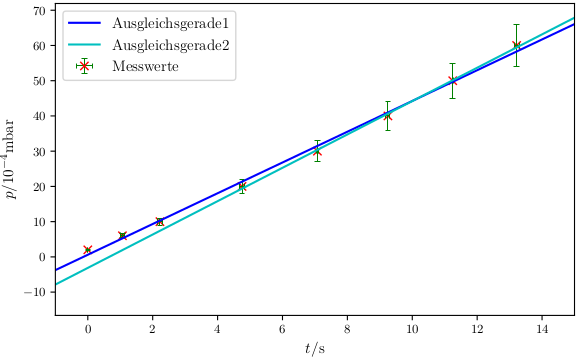
\includegraphics[width=\linewidth-70pt,height=\textheight-70pt,keepaspectratio]{content/images/TL1.png}
\caption{Der Druck $p$ in Abhängigkeit von der mittleren Zeit $\bar{t}$ bei der Leckratenmessung der Turbopumpe  mit $p_.g = \SI{2e-4}{\milli\bar}$.}
\label{fig:TL1}
\end{figure}

\begin{table}
\centering
\caption{Die Messwerte der Leckratenmessung bei der Turborpumpe mit einem Gleichgewichtsdruck von $p_.g = \SI{1.4e-4}{\milli\bar}$.}
\label{tab:tabTL2}
	\sisetup{table-format=1.2}
	\begin{tabular}{S[table-format=2.0] @{${}\pm{}$} S[table-format=1.1]S[table-format=2.2]S[table-format=2.2]S[table-format=2.2]S[table-format=2.2] @{${}\pm{}$} S[table-format=1.2]}
		\toprule
		\multicolumn{2}{c}{$p/10^{-4}\si{\milli\bar}$} & {$t_1/\si{\second}$} & {$t_2/\si{\second}$} & {$t_3/\si{\second}$} & \multicolumn{2}{c}{$\bar{t}/\si{\second}$} \\
		\midrule
		 6 & 0.6 & 2.06 & 2.15 & 2.13 & 2.11 & 0.03 \\
		10 & 1.0 & 3.64 & 3.81 & 3.81 & 3.75 & 0.06 \\
		20 & 2.0 & 7.57 & 7.45 & 7.49 & 7.50 & 0.04 \\
		30 & 3.0 & 10.68 & 10.75 & 10.62 & 10.68 & 0.04 \\
		40 & 4.0 & 13.66 & 13.80 & 13.88 & 13.78 & 0.06 \\
		50 & 5.0 & 16.62 & 16.86 & 16.76 & 16.75 & 0.07 \\
		60 & 6.0 & 19.48 & 19.66 & 19.66 & 19.60 & 0.06 \\
		\bottomrule
	\end{tabular}

\label{tab:TL2}
\end{table}

\begin{figure}
\centering
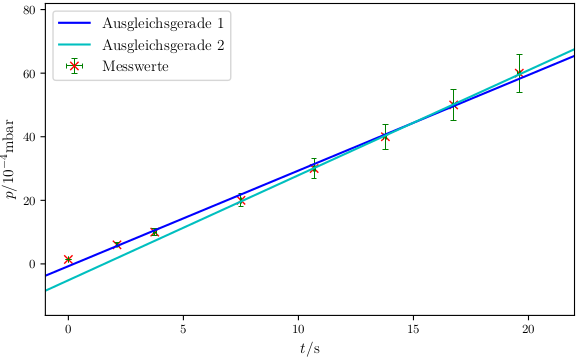
\includegraphics[width=\linewidth-70pt,height=\textheight-70pt,keepaspectratio]{content/images/TL2.png}
\caption{Der Druck $p$ in Abhängigkeit von der mittleren Zeit $\bar{t}$ bei der Leckratenmessung der Turbopumpe  mit $p_.g = \SI{1.4e-4}{\milli\bar}$.}
\label{fig:TL2}
\end{figure}

\begin{table}
\centering
\caption{Die Messwerte der Leckratenmessung bei der Turborpumpe mit einem Gleichgewichtsdruck von $p_.g = \SI{1e-4}{\milli\bar}$.}
\label{tab:tabTL3}
	\sisetup{table-format=1.2}
	\begin{tabular}{S[table-format=2.0] @{${}\pm{}$} S[table-format=1.1]S[table-format=2.2]S[table-format=2.2]S[table-format=2.2]S[table-format=2.2] @{${}\pm{}$} S[table-format=1.2]}
		\toprule
		\multicolumn{2}{c}{$p/10^{-4}\si{\milli\bar}$} & {$t_1/\si{\second}$} & {$t_2/\si{\second}$} & {$t_3/\si{\second}$} & \multicolumn{2}{c}{$\bar{t}/\si{\second}$} \\
		\midrule
		 1 & 0.1 & 0.00 & 0.00 & 0.00 & 0.00 & 0.00 \\
		 4 & 0.4 & 1.43 & 1.78 & 1.55 & 1.59 & 0.11 \\
		 8 & 0.8 & 3.66 & 4.14 & 3.93 & 3.91 & 0.14 \\
		20 & 2.0 & 9.54 & 10.17 & 9.93 & 9.88 & 0.19 \\
		30 & 3.0 & 14.28 & 14.46 & 14.59 & 14.44 & 0.09 \\
		40 & 4.0 & 18.39 & 18.84 & 18.92 & 18.72 & 0.17 \\
		50 & 5.0 & 22.50 & 22.85 & 23.00 & 22.78 & 0.15 \\
		60 & 6.0 & 26.23 & 26.69 & 26.68 & 26.53 & 0.16 \\
		70 & 7.0 & 29.88 & 30.37 & 30.38 & 30.21 & 0.17 \\
		\bottomrule
	\end{tabular}

\label{tab:TL3}
\end{table}

\begin{figure}
\centering
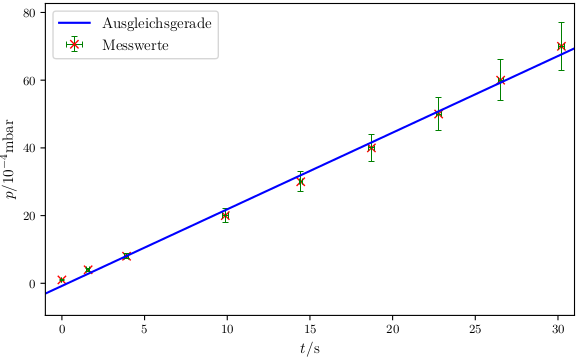
\includegraphics[width=\linewidth-70pt,height=\textheight-70pt,keepaspectratio]{content/images/TL3.png}
\caption{Der Druck $p$ in Abhängigkeit von der mittleren Zeit $\bar{t}$ bei der Leckratenmessung der Turbopumpe  mit $p_.g = \SI{1e-4}{\milli\bar}$.}
\label{fig:TL3}
\end{figure}

\begin{table}
\centering
\caption{Die Messwerte der Leckratenmessung bei der Turborpumpe mit einem Gleichgewichtsdruck von $p_.g = \SI{0.5e-4}{\milli\bar}$.}
\label{tab:tabTL4}
	\sisetup{table-format=1.2}
	\begin{tabular}{S[table-format=2.0] @{${}\pm{}$} S[table-format=1.1]S[table-format=2.2]S[table-format=2.2]S[table-format=2.2]S[table-format=2.2] @{${}\pm{}$} S[table-format=1.2]}
		\toprule
		\multicolumn{2}{c}{$p/10^{-4}\si{\milli\bar}$} & {$t_1/\si{\second}$} & {$t_2/\si{\second}$} & {$t_3/\si{\second}$} & \multicolumn{2}{c}{$\bar{t}/\si{\second}$} \\
		\midrule
		 2 & 0.2 & 2.25 & 2.15 & 2.41 & 2.27 & 0.08 \\
		 3 & 0.3 & 3.83 & 3.66 & 4.00 & 3.83 & 0.10 \\
		 4 & 0.4 & 5.43 & 5.12 & 5.44 & 5.33 & 0.11 \\
		 5 & 0.5 & 6.94 & 6.61 & 6.92 & 6.82 & 0.11 \\
		 6 & 0.6 & 8.42 & 8.11 & 8.40 & 8.31 & 0.10 \\
		 7 & 0.7 & 9.95 & 9.56 & 9.85 & 9.79 & 0.12 \\
		 8 & 0.8 & 11.36 & 10.99 & 11.23 & 11.19 & 0.11 \\
		 9 & 0.9 & 12.85 & 12.38 & 12.62 & 12.62 & 0.14 \\
		10 & 1.0 & 14.34 & 13.78 & 14.07 & 14.06 & 0.16 \\
		20 & 2.0 & 28.07 & 26.68 & 27.37 & 27.37 & 0.40 \\
		\bottomrule
	\end{tabular}

\label{tab:TL4}
\end{table}

\begin{figure}
\centering
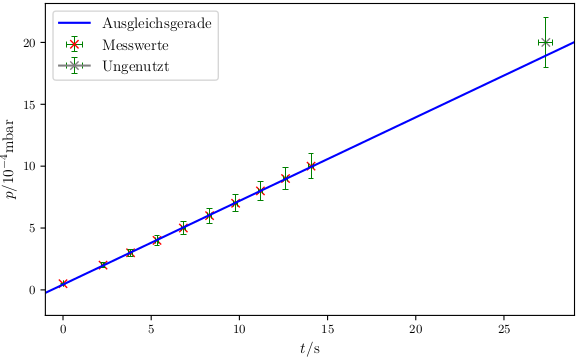
\includegraphics[width=\linewidth-70pt,height=\textheight-70pt,keepaspectratio]{content/images/TL4.png}
\caption{Der Druck $p$ in Abhängigkeit von der mittleren Zeit $\bar{t}$ bei der Leckratenmessung der Turbopumpe  mit $p_.g = \SI{0.5e-4}{\milli\bar}$.}
\label{fig:TL4}
\end{figure}

\subsubsection{Bestimmung des Saugvermögens $S$ über die Evakuierungskurve}

In Tabelle \ref{tab:TS} sind die Messwerte für die Evakuierungskurve, sowie die nach Formel \eqref{eq:tQuer} berechneten Mittelwerte $\bar{t}$ eingetragen.
Dabei entsprechen $p_0=\SI{500(100)e-5}{\milli\bar}$ dem Anfangsdruck und $p_.E=\SI{1.2(2)e-5}{\milli\bar}$ dem Enddruck der Kurve. Der Fehler des Druckes ergibt sich aus der Ungenauigkeit der Messskala von $20\%$ \cite{V70}. 
Der Fehler der logarithmischen Werte berechnet sich nach der Gaußschen Fehlerfortpflanzung:
\[
\sigma_f = \sqrt{\sum_i\left(\frac{\partial f}{\partial x_i}\sigma_{x_i}\right)^2}\text{.}
\]
Konkret:
\begin{align*}
\sigma_.{ln}	&=\sqrt{\frac{\sigma_p^2+\sigma_{p_.E}^2}{(p-p_.E)^2}+\frac{\sigma_{p_0}^2+\sigma_{p_.E}^2}{(p_0-p_.E)^2}}\text{.} \label{eq:ln}
%\sigma_.{ln}	&=\frac{1}{z}\sigma_{z}\text{;}\\
%z				&=\frac{p-p_.E}{p_0-p_.E}\text{,}\\
%\sigma_{z}	&=\sqrt{\left(\frac{1}{p_y}\sigma_{p_x}\right)^2+\left(\frac{p_x}{p_y^2}\sigma_{p_y}\right)^2}\text{;}\\
%p_x				&=p-p_.E\text{,}\\
%p_y				&=p_0-p_.E\text{,}\\
%\sigma_{p_x}	&=\sqrt{\sigma_p^2+\sigma_{p_.E}^2}\text{,}\\
%\sigma_{p_y}	&=\sqrt{\sigma_{p_0}^2+\sigma_{p_.E}^2}\text{.}\\
\end{align*}
Dabei entsprechen die $\sigma_{p_i}$ den jeweiligen Abweichungen der $p_i$.
Die Evakuierungskurve ist in Abbildung \ref{fig:TSE} zu sehen, die logarithmische Darstellung in Abbildung \ref{fig:TSL}.
Lineare Ausgleichsrechnungen der Form
\[
\ln\left(\frac{p(t)-p_.E}{p_0-p_.E}\right) = a_it+b_i
\]
für die ersten vier Messwerte (Ausgleichsgerade 1), den fünften bis achten Messwert (Ausgleichsgerade 2) und den siebten bis zehnten Messwert (Ausgleichsgerade 3) ergeben die Parameter:
\begin{align*}
a_.{TE1} &= \SI{-0.89(2)}{\per\second} \text{,}\\
b_.{TE1} &= \SI{-0.05(5)}{} \text{,}\\
a_.{TE2} &= \SI{-0.51(4)}{\per\second} \text{,}\\
b_.{TE2} &= \SI{-1.9(3)}{} \text{,}\\
a_.{TE3} &= \SI{-0.21(3)}{\per\second} \text{,}\\
b_.{TE3} &= \SI{-4.6(3)}{} \text{.}\\
\end{align*} 
Daraus folgen mit Formel \eqref{eq:S} für $S$ die Werte:
\begin{align*}
S_.{TE1} &= \SI{9.1(8)}{\litre\per\second} \text{,}\\
S_.{TE2} &= \SI{5.2(6)}{\litre\per\second} \text{,}\\
S_.{TE3} &= \SI{2.2(3)}{\litre\per\second} \text{.}\\
\end{align*} 
Das benötigte Volumen $V_.{TE}$ bestimmt sich dabei mit den Werten aus Tabelle \ref{tab:V} zu:
\[
V_.{TE} = \SI{10.3(9)}{\litre}\text{.}
\]

\begin{table}
\centering
\caption{Die Werte für die Evakuierungskurve der Turborpumpe.}
\label{tab:tabTS}
	\sisetup{table-format=1.2}
	\begin{tabular}{S[table-format=3.1] @{${}\pm{}$} S[table-format=2.1]S[table-format=2.1] @{${}\pm{}$} S[table-format=1.1]S[table-format=2.2]S[table-format=2.2]S[table-format=2.2]S[table-format=2.2]S[table-format=2.2]S[table-format=2.2]S[table-format=2.2] @{${}\pm{}$} S[table-format=1.2]}
		\toprule
		\multicolumn{2}{c}{$p/10^{-5}\si{\milli\bar}$} & \multicolumn{2}{c}{$\log\left(\frac{p-p_e}{p_0-p_e}\right)$} & {$t_1/\si{\second}$} & {$t_2/\si{\second}$} & {$t_3/\si{\second}$} & {$t_4/\si{\second}$} & {$t_5/\si{\second}$} & {$t_6/\si{\second}$} & \multicolumn{2}{c}{$\bar{t}/\si{\second}$} \\
		\midrule
		500.0 & 50.0 & 0.0 & 0.0 & 0.00 & 0.00 & 0.00 & 0.00 & 0.00 & 0.00 & 0.00 & 0.00 \\
		200.0 & 20.0 & -0.9 & 0.2 & 0.86 & 0.98 & 0.90 & 0.93 & 0.81 & 1.03 & 0.92 & 0.04 \\
		40.0 & 4.0 & -2.6 & 0.2 & 2.72 & 2.82 & 2.71 & 2.89 & 2.71 & 2.98 & 2.81 & 0.05 \\
		20.0 & 2.0 & -3.3 & 0.2 & 3.57 & 3.78 & 3.51 & 3.80 & 3.54 & 3.84 & 3.67 & 0.07 \\
		6.0 & 0.6 & -4.6 & 0.2 & 5.55 & 5.69 & 5.50 & 5.66 & 5.47 & 5.82 & 5.61 & 0.06 \\
		4.0 & 0.4 & -5.2 & 0.2 & 6.31 & 6.48 & 6.28 & 6.69 & 6.31 & 6.60 & 6.45 & 0.08 \\
		2.0 & 0.2 & -6.4 & 0.4 & 8.66 & 8.89 & 8.71 & 8.75 & 8.69 & 9.18 & 8.81 & 0.09 \\
		1.8 & 0.2 & -6.7 & 0.4 & 9.82 & 9.80 & 9.76 & 9.66 & 9.40 & 10.24 & 9.78 & 0.12 \\
		1.6 & 0.2 & -7.1 & 0.6 & 11.01 & 11.13 & 11.34 & 10.64 & 10.56 & 11.40 & 11.01 & 0.15 \\
		1.4 & 0.2 & -7.8 & 1.0 & 15.24 & 15.19 & 15.34 & 14.85 & 14.59 & 15.45 & 15.11 & 0.14 \\
		\bottomrule
	\end{tabular}

\label{tab:TS}
\end{table}

\begin{figure}
\centering
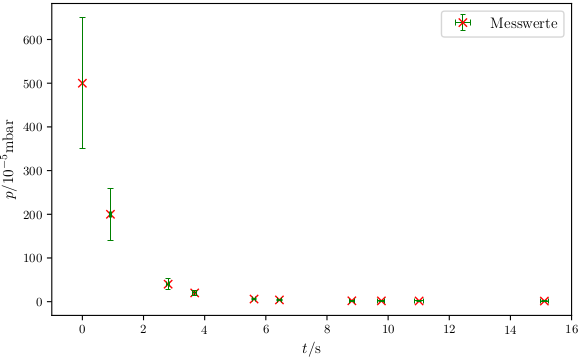
\includegraphics[width=\linewidth-70pt,height=\textheight-70pt,keepaspectratio]{content/images/TSE.png}
\caption{Die Evakuierungskurve der Turbopumpe.}
\label{fig:TSE}
\end{figure}

\begin{figure}
\centering
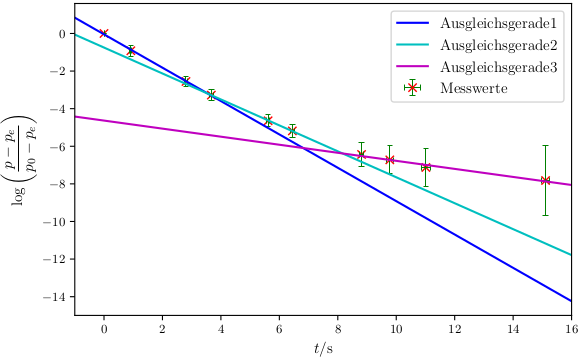
\includegraphics[width=\linewidth-70pt,height=\textheight-70pt,keepaspectratio]{content/images/TSL.png}
\caption{Die logarithmische Evakuierungskurve der Turbopumpe.}
\label{fig:TSL}
\end{figure}

\subsection{Drehschieberpumpe}

\subsubsection{Bestimmung des Saugvermögens $S$ über die Leckratenmessung}

Die Leckratenmessung wurde bei vier unterschiedlichen Gleichgewichtsdrücken $p_.g$ durchgeführt. Dabei werden die gemessenen Zeiten $t_i$ mit Formel \eqref{eq:tQuer} gemittelt.
In den Tabellen \ref{tab:DL1} bis \ref{tab:DL4} sind die Messwerte und die zugehörigen Mittelwerte der jeweiligen Messreihen aufgelistet. Der Fehler des Druckes ergibt sich dabei aus der Ungenauigkeit der Messskala von $10\%$ \cite{V70}.\\
In den Abbildungen \ref{fig:DL1} bis \ref{fig:DL4} ist der Druck $p$ gegen die gemittelte Zeit $\bar{t}$ aufgetragen.
Die linearen Ausgleichsrechnungen der Form
\[
p_i(t) = a_it+b_i
\]
ergeben für $p_.g = \SI{1}{\milli\bar}$ die Parameter
\begin{align*}
a_.{DL1} &= \SI{0.122(2)}{\milli\bar\per\second} \text{,}\\
b_.{DL1} &= \SI{0.91(6)}{\milli\bar} \text{,}\\
\end{align*}
für $p_g = \SI{0.8}{\milli\bar}$
\begin{align*}
a_.{DL2} &= \SI{0.098(2)}{\milli\bar\per\second} \text{,}\\
b_.{DL2} &= \SI{0.77(6)}{\milli\bar} \text{,}\\
\end{align*}
für $p_g = \SI{0.4}{\milli\bar}$
\begin{align*}
a_.{DL3} &= \SI{0.034(1)}{\milli\bar\per\second} \text{,}\\
b_.{DL3} &= \SI{0.25(9)}{\milli\bar} \text{,}\\
\end{align*}
und für $p_g = \SI{0.1}{\milli\bar}$
\begin{align*}
a_.{DL4} &= \SI{0.0048(2)}{\milli\bar\per\second} \text{,}\\
b_.{DL4} &= \SI{0.14(2)}{\milli\bar} \text{.}
\end{align*}
In den Graphen sind die nicht genutzten Messwerte Grau markiert.
Mit Formel \eqref{eq:S2} ergibt sich für das Saugvermögen $S$
\begin{align*}
S_.{DL1} &= \SI{1.4(1)}{\litre\per\second} \text{,}\\
S_.{DL2} &= \SI{1.4(1)}{\litre\per\second} \text{,}\\
S_.{DL3} &= \SI{0.95(9)}{\litre\per\second} \text{,}\\
S_.{DL4}   &= \SI{0.53(5)}{\litre\per\second} \text{.}
\end{align*}
Das benötigte Volumen $V_.{DL}$ bestimmt sich dabei mit den Werten aus Tabelle \ref{tab:V} zu:
\[
V_.{DL} = \SI{11(1)}{\litre}\text{.}
\]


\begin{table}
\centering
\caption{Die Messwerte der Leckratenmessung bei der Drehschieberpumpe mit einem Gleichgewichtsdruck von $p_.g = \SI{1}{\milli\bar}$.}
\label{tab:tabDL1}
	\sisetup{table-format=1.2}
	\begin{tabular}{S[table-format=2.0] @{${}\pm{}$} S[table-format=1.1]S[table-format=2.2]S[table-format=2.2]S[table-format=2.2]S[table-format=2.2]S[table-format=2.2] @{${}\pm{}$} S[table-format=1.2]}
		\toprule
		\multicolumn{2}{c}{$p/\si{\milli\bar}$} & {$t_1/\si{\second}$} & {$t_2/\si{\second}$} & {$t_3/\si{\second}$} & {$t_4/\si{\second}$} & \multicolumn{2}{c}{$\bar{t}/\si{\second}$} \\
		\midrule
		 2 & 0.4 & 8.91 & 9.81 & 10.36 & 9.55 & 9.66 & 0.30 \\
		 4 & 0.8 & 25.87 & 25.15 & 27.01 & 26.21 & 26.06 & 0.39 \\
		 6 & 1.2 & 40.78 & 41.33 & 42.06 & 40.74 & 41.23 & 0.31 \\
		 8 & 1.6 & 57.78 & 58.09 & 56.92 & 57.58 & 57.59 & 0.25 \\
		10 & 2.0 & 74.33 & 75.40 & 76.27 & 73.51 & 74.88 & 0.60 \\
		\bottomrule
	\end{tabular}

\label{tab:DL1}
\end{table}

\begin{figure}
\centering
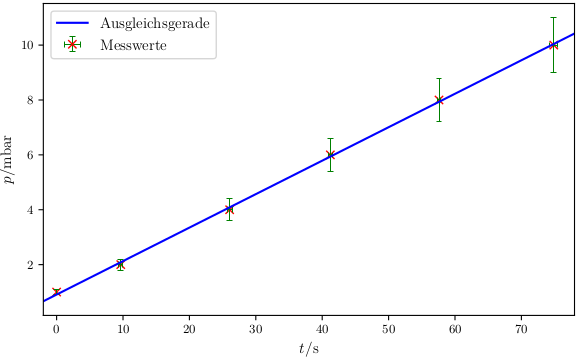
\includegraphics[width=\linewidth-70pt,height=\textheight-70pt,keepaspectratio]{content/images/DL1.png}
\caption{Der Druck $p$ in Abhängigkeit von der mittleren Zeit $\bar{t}$ bei der Leckratenmessung der Drehschieberpumpe  mit $p_.g = \SI{1}{\milli\bar}$.}
\label{fig:DL1}
\end{figure}

\begin{table}
\centering
\caption{Die Messwerte der Leckratenmessung bei der Drehschieberpumpe mit einem Gleichgewichtsdruck von $p_.g = \SI{0.8}{\milli\bar}$.}
\label{tab:tabDL2}
	\sisetup{table-format=1.2}
	\begin{tabular}{S[table-format=2.0] @{${}\pm{}$} S[table-format=1.1]S[table-format=2.2]S[table-format=2.2]S[table-format=2.2]S[table-format=2.2] @{${}\pm{}$} S[table-format=1.2]}
		\toprule
		\multicolumn{2}{c}{$p/\si{\milli\bar}$} & {$t_1/\si{\second}$} & {$t_2/\si{\second}$} & {$t_3/\si{\second}$} & \multicolumn{2}{c}{$\bar{t}/\si{\second}$} \\
		\midrule
		 2 & 0.4 & 12.28 & 11.88 & 12.29 & 12.15 & 0.14 \\
		 4 & 0.8 & 33.98 & 35.09 & 33.67 & 34.25 & 0.44 \\
		 6 & 1.3 & 52.83 & 52.47 & 52.65 & 52.65 & 0.11 \\
		 8 & 1.6 & 73.54 & 73.97 & 73.18 & 73.56 & 0.23 \\
		10 & 2.0 & 76.73 & 76.87 & 75.98 & 76.53 & 0.28 \\
		\bottomrule
	\end{tabular}

\label{tab:DL2}
\end{table}

\begin{figure}
\centering
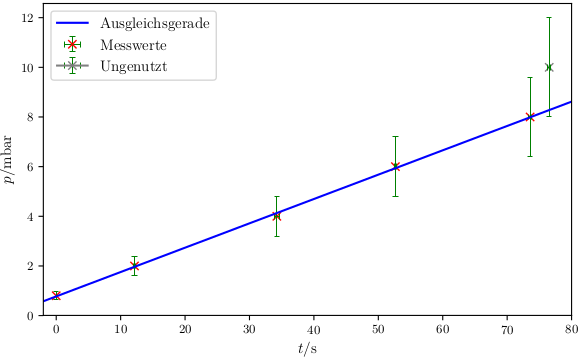
\includegraphics[width=\linewidth-70pt,height=\textheight-70pt,keepaspectratio]{content/images/DL2.png}
\caption{Der Druck $p$ in Abhängigkeit von der mittleren Zeit $\bar{t}$ bei der Leckratenmessung der Drehschieberpumpe  mit $p_.g = \SI{0.8}{\milli\bar}$.}
\label{fig:DL2}
\end{figure}

\begin{table}
\centering
\caption{Die Messwerte der Leckratenmessung bei der Drehschieberpumpe mit einem Gleichgewichtsdruck von $p_.g = \SI{0.4}{\milli\bar}$.}
\label{tab:tabDL3}
	\sisetup{table-format=1.2}
	\begin{tabular}{S[table-format=1.1] @{${}\pm{}$} S[table-format=1.1]S[table-format=2.2]S[table-format=2.2]S[table-format=2.2]S[table-format=2.2] @{${}\pm{}$} S[table-format=1.2]}
		\toprule
		\multicolumn{2}{c}{$p/\si{\milli\bar}$} & {$t_1/\si{\second}$} & {$t_2/\si{\second}$} & {$t_3/\si{\second}$} & \multicolumn{2}{c}{$\bar{t}/\si{\second}$} \\
		\midrule
		0.6 & 0.1 & 8.28 & 9.35 & 8.71 & 8.78 & 0.31 \\
		1.0 & 0.1 & 23.33 & 23.89 & 23.85 & 23.69 & 0.18 \\
		2.0 & 0.2 & 57.47 & 56.65 & 55.97 & 56.70 & 0.43 \\
		4.0 & 0.4 & 113.70 & 113.33 & 112.68 & 113.24 & 0.30 \\
		6.0 & 0.6 & 164.21 & 165.51 & 165.13 & 164.95 & 0.39 \\
		\bottomrule
	\end{tabular}

\label{tab:DL3}
\end{table}

\begin{figure}
\centering
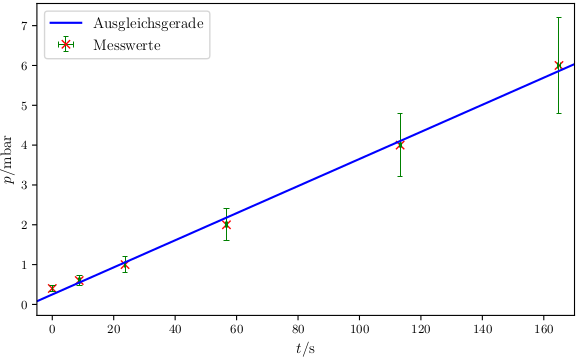
\includegraphics[width=\linewidth-70pt,height=\textheight-70pt,keepaspectratio]{content/images/DL3.png}
\caption{Der Druck $p$ in Abhängigkeit von der mittleren Zeit $\bar{t}$ bei der Leckratenmessung der Drehschieberpumpe  mit $p_.g = \SI{0.4}{\milli\bar}$.}
\label{fig:DL3}
\end{figure}

\begin{table}
\centering
\caption{Die Messwerte der Leckratenmessung bei der Drehschieberpumpe mit einem Gleichgewichtsdruck von $p_.g = \SI{0.1}{\milli\bar}$.}
\label{tab:tabDL4}
	\sisetup{table-format=1.2}
	\begin{tabular}{S[table-format=1.1] @{${}\pm{}$} S[table-format=1.2]S[table-format=2.2]S[table-format=2.2]S[table-format=2.2]S[table-format=2.2] @{${}\pm{}$} S[table-format=1.2]}
		\toprule
		\multicolumn{2}{c}{$p/\si{\milli\bar}$} & {$t_1/\si{\second}$} & {$t_2/\si{\second}$} & {$t_3/\si{\second}$} & \multicolumn{2}{c}{$\bar{t}/\si{\second}$} \\
		\midrule
		0.2 & 0.05 & 9.95 & 10.08 & 10.66 & 10.23 & 0.22 \\
		0.4 & 0.09 & 46.08 & 46.54 & 46.48 & 46.37 & 0.15 \\
		0.6 & 0.12 & 93.01 & 95.29 & 95.11 & 94.47 & 0.74 \\
		0.8 & 0.17 & 141.51 & 141.29 & 142.19 & 141.66 & 0.28 \\
		1.0 & 0.20 & 179.62 & 180.72 & 180.07 & 180.14 & 0.32 \\
		\bottomrule
	\end{tabular}

\label{tab:DL4}
\end{table}

\begin{figure}
\centering
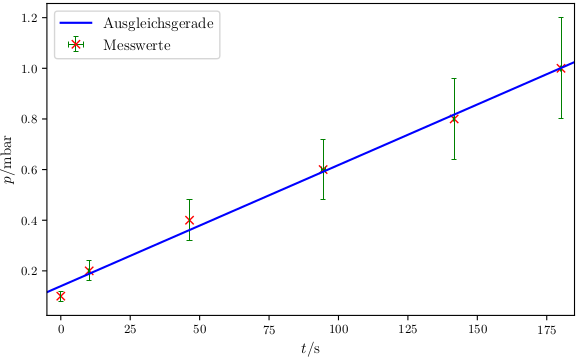
\includegraphics[width=\linewidth-70pt,height=\textheight-70pt,keepaspectratio]{content/images/DL4.png}
\caption{Der Druck $p$ in Abhängigkeit von der mittleren Zeit $\bar{t}$ bei der Leckratenmessung der Drehschieberpumpe  mit $p_.g = \SI{0.1}{\milli\bar}$.}
\label{fig:DL4}
\end{figure}

\subsubsection{Bestimmung des Saugvermögens $S$ über die Evakuierungskurve}

In Tabelle \ref{tab:DS} sind die Messwerte für die Evakuierungskurve, sowie die nach Formel \eqref{eq:tQuer} berechneten Mittelwerte $\bar{t}$ eingetragen.
Dabei entsprechen $p_0=\SI{1013}{\milli\bar}$ dem Anfangsdruck und $p_.E=\SI{0.02}{\milli\bar}$ dem Enddruck der Kurve. Der Fehler des Druckes ergibt sich aus der Ungenauigkeit der Messskala von $20\%$ \cite{V70}. 
Der Fehler der logarithmischen Werte berechnet sich nach Formel \eqref{eq:ln}.
Die Evakuierungskurve ist in Abbildung \ref{fig:DSE} zu sehen, die logarithmische Darstellung in Abbildung \ref{fig:DSL}.
Lineare Ausgleichsrechnungen der Form
\[
\ln\left(\frac{p(t)-p_.E}{p_0-p_.E}\right) = a_it+b_i
\]
für die ersten elf Messwerte (Ausgleichsgerade 1) und den zwöften bis siebzehnten Messwert (Ausgleichsgerade 2) ergeben die Parameter:
\begin{align*}
a_.{DE1} &= \SI{-0.093(2)}{\per\second} \text{,}\\
b_.{DE1} &= \SI{-0.08(8)}{} \text{,}\\
a_.{DE2} &= \SI{-0.0619(8)}{\per\second} \text{,}\\
b_.{DE2} &= \SI{-2.51(8)}{} \text{,}\\
\end{align*} 
Daraus folgen mit Formel \eqref{eq:} für $S$ die Werte:
\begin{align*}
S_.{DE1} &= \SI{1.0(1)}{\litre\per\second} \text{,}\\
S_.{DE2} &= \SI{0.69(6)}{\litre\per\second} \text{.}\\
\end{align*} 
Das benötigte Volumen $V_.{TE}$ bestimmt sich dabei mit den Werten aus Tabelle \ref{tab:V} zu:
\[
V_.{DE} = \SI{11.1(1)}{\litre}\text{.}
\]

\begin{table}
\centering
\caption{Die Werte für die Evakuierungskurve der Drehschieberpumpe.}
\label{tab:tabDS}
	\sisetup{table-format=1.2}
	\begin{tabular}{S[table-format=3.2] @{${}\pm{}$} S[table-format=2.2]S[table-format=3.1] @{${}\pm{}$} S[table-format=1.1]S[table-format=3.2]S[table-format=3.2]S[table-format=3.2]S[table-format=3.2]S[table-format=3.2]S[table-format=3.2]@{${}\pm{}$} S[table-format=1.2]}
		\toprule
		\multicolumn{2}{c}{$p/\si{\milli\bar}$} & \multicolumn{2}{c}{$\log\left(\frac{p-p_e}{p_0-p_e}\right)$} & {$t_1/\si{\second}$} & {$t_2/\si{\second}$} & {$t_3/\si{\second}$} & {$t_4/\si{\second}$} & {$t_5/\si{\second}$} & \multicolumn{2}{c}{$\bar{t}/\si{\second}$} \\
		\midrule
		100.00 & 20.00 & -2.3 & 0.3 & 18.81 & 21.62 & 21.50 & 21.49 & 22.65 & 21.21 & 0.64 \\
		60.00 & 12.00 & -2.8 & 0.3 & 28.25 & 30.40 & 29.56 & 29.04 & 29.66 & 29.38 & 0.36 \\
		40.00 & 8.00 & -3.2 & 0.3 & 34.20 & 35.60 & 34.94 & 34.60 & 35.09 & 34.89 & 0.24 \\
		20.00 & 4.00 & -3.9 & 0.3 & 41.58 & 42.91 & 42.67 & 42.14 & 42.74 & 42.41 & 0.24 \\
		10.00 & 2.00 & -4.6 & 0.3 & 48.64 & 50.71 & 50.13 & 49.57 & 50.15 & 49.84 & 0.35 \\
		8.00 & 1.60 & -4.8 & 0.3 & 51.02 & 52.75 & 52.53 & 51.62 & 52.26 & 52.04 & 0.32 \\
		6.00 & 1.20 & -5.1 & 0.3 & 54.26 & 55.95 & 55.67 & 55.18 & 55.54 & 55.32 & 0.29 \\
		4.00 & 0.80 & -5.5 & 0.3 & 57.89 & 59.43 & 59.56 & 58.78 & 59.44 & 59.02 & 0.31 \\
		2.00 & 0.40 & -6.2 & 0.3 & 64.57 & 66.21 & 66.08 & 65.64 & 66.19 & 65.74 & 0.31 \\
		1.00 & 0.20 & -6.9 & 0.3 & 71.90 & 73.67 & 73.49 & 73.12 & 73.60 & 73.16 & 0.33 \\
		0.80 & 0.16 & -7.2 & 0.3 & 74.34 & 75.85 & 76.00 & 75.51 & 75.98 & 75.54 & 0.31 \\
		0.60 & 0.12 & -7.5 & 0.3 & 78.49 & 80.16 & 80.20 & 79.46 & 80.18 & 79.70 & 0.33 \\
		0.40 & 0.08 & -7.9 & 0.3 & 85.43 & 87.42 & 86.81 & 86.62 & 87.16 & 86.69 & 0.34 \\
		0.20 & 0.04 & -8.6 & 0.3 & 98.56 & 99.93 & 99.71 & 99.35 & 99.56 & 99.42 & 0.24 \\
		0.10 & 0.02 & -9.4 & 0.3 & 110.69 & 111.87 & 111.74 & 110.95 & 111.57 & 111.36 & 0.23 \\
		0.08 & 0.02 & -9.7 & 0.3 & 116.74 & 117.48 & 116.94 & 116.99 & 116.93 & 117.02 & 0.12 \\
		0.06 & 0.01 & -10.1 & 0.4 & 129.17 & 129.04 & 128.40 & 127.59 & 128.66 & 128.57 & 0.28 \\
		\bottomrule
	\end{tabular}

\label{tab:DS}
\end{table}

\begin{figure}
\centering
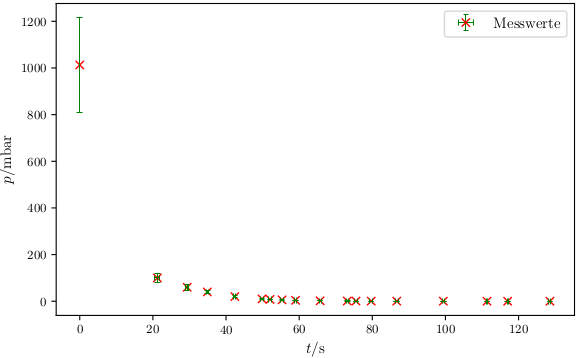
\includegraphics[width=\linewidth-70pt,height=\textheight-70pt,keepaspectratio]{content/images/DSE.png}
\caption{Die Evakuierungskurve der Drehschieberpumpe.}
\label{fig:DSE}
\end{figure}

\begin{figure}
\centering
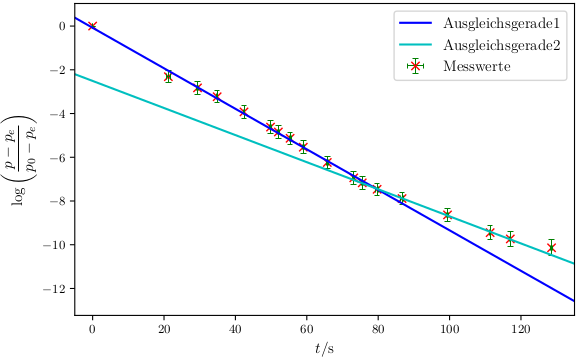
\includegraphics[width=\linewidth-70pt,height=\textheight-70pt,keepaspectratio]{content/images/DSL.png}
\caption{Die logarithmische Evakuierungskurve der Drehschieberpumpe.}
\label{fig:DSL}
\end{figure}

\subsection{Zusammenfassung} 

In den Abbildungen \ref{fig:TGes} und \ref{fig:DGes} sind die Ergebnisse für das Saugvermögen der jeweiligen Pumpe gegen den Druck aufgetragen. Die Bezeichnungen in der Legende beziehen sich dabei auf die Indizes der Werte.\\
Die Werte aus der Leckratenmessung sind als Punkte dargestellt, die Werte aus der Evakuierungskurve als gestrichelte Linie zwischen dem Anfangs- und Endpunkt des jeweiligen Druckbereichs. Da der Druckbereich der TS1- und DS1-Linie vergleichsweise sehr groß ist, sind die Graphen rechts abgeschnitten. 

\begin{figure}
\centering
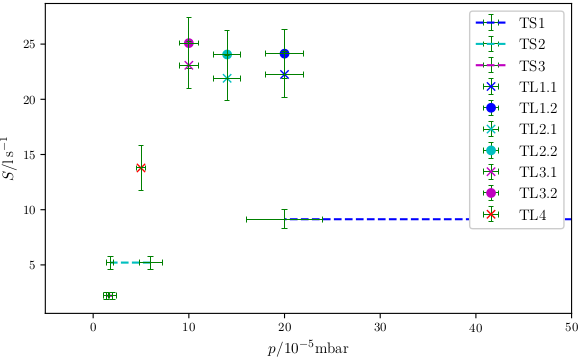
\includegraphics[width=\linewidth-70pt,height=\textheight-70pt,keepaspectratio]{content/images/TGes.png}
\caption{Das Saugvermögen $S$ der Turbomoolekularpumpe in Abhängigkeit vom Druck $p$.}
\label{fig:TGes}
\end{figure}

\begin{figure}
\centering
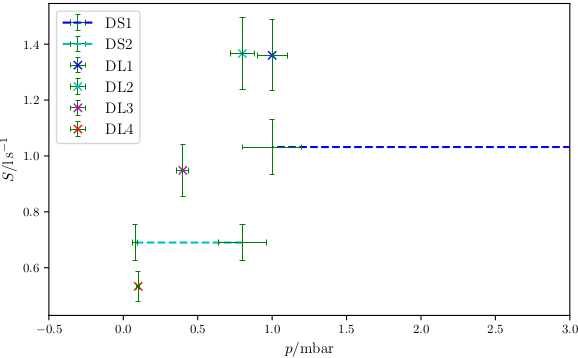
\includegraphics[width=\linewidth-70pt,height=\textheight-70pt,keepaspectratio]{content/images/DGes.png}
\caption{Das Saugvermögen $S$ der Drehschieberpumpe in Abhängigkeit vom Druck $p$.}
\label{fig:DGes}
\end{figure}